\documentclass{article}

%% Page Margins %%
\usepackage{geometry}
\geometry{
    top = 0.75in,
    bottom = 0.75in,
    right = 0.75in,
    left = 0.75in,
}

\usepackage{amsmath}
\usepackage{graphicx}
\usepackage{parskip}

\title{Project Report: Milestone 1}

\author{Janssen Myer Rambaud (1008107004), Felix Zhang (1007650212)}

\begin{document}
\maketitle

\section{Part I: Planning and Configuration}

\begin{enumerate}
\item \textbf{Breakout Bitmap Display and Memory Map Plan}: 
Our plan is to have a 512 pixel (wdith) x 256 pixel (height) display while keeping the same base address 0x10008000 (\$gp). We also plan on having unit widths be 4 pixels x 4 pixels because it remains even while being a better size than say 2 x 2, which is too small. Table is on the next page.

\begin{table}[]
\begin{tabular}{|l|l|l|}
\hline
Data Segment     & Address                                                           & Data           \\ \hline
IMMUTABLE DATA   &                                                                   &                \\ \hline
                 & 0x10008000 (Address of Bitmap Display)                            & ADDR\_DSPL    \\ \hline
                 & 0xffff0000 (Address of Keyboard)                                  & ADDR\_KBRD     \\ \hline
                 & Takes in 1 address (Display width divided by unit width [in pixels])           & SCREEN\_WIDTH  \\ \hline
                 & Takes in 2 addresses for (length, height) of the paddle                                           & PADDLE\_DIM    \\ \hline
                 & Takes in 1 address for width of wall                                           & WALL\_WIDTH    \\ \hline
                 & Takes in 2 addresses (left wall x-coordinate, right wall x-coordinate) for paddle collision                                 & WALLS\_X     \\ \hline
                                  & Takes in 1 address for (height) of buffer                                                           & BUFFER\_HEIGHT \\ \hline
                 & Takes in 1 address buffer colour (used for drawing walls, bricks)              & BUFFER\_COLOUR \\ \hline
                                  & Takes in 1 address for the y coordinate of a brick                & BRICKS\_Y      \\ \hline
                 & Takes in 2 addresses (2-D array that stores colour)               & BRICKS         \\ \hline
                 & Takes in 2 addresses (width, height) for a brick               & BRICKS\_DIM         \\ \hline
                 & Takes in 7 addresses (1 for array length, 6 for elements/colours) & COLOURS        \\ \hline
MUTABLE DATA     &                                                                   &                \\ \hline
                                  & Takes in 1 address for colour of paddle (gray)                                 & PADDLE\_COLOUR \\ \hline
                 & Takes in 1 address for colour of ball (white)                                  & BALL\_COLOUR   \\ \hline
                 & Takes in 2 addresses (x, y) coordinates                           & PADDLE\_COORDS \\ \hline
                 & Takes in 2 addresses (x, y) coordinates                           & BALL\_COORDS   \\ \hline
                 & Takes in 1 address for the movement direction of the ball         & DIRECTION      \\ \hline
\end{tabular}
\end{table}

\\

\newpage
\item Translate your plan into the .data section of your breakout.asm program. Assemble your program in MARS and inspect memory to ensure it matches your plan. Include a screenshot (or multiple screenshots) of memory demonstrating that it has been laid out according to your plan.

\begin{figure}[ht!]
    \centering
    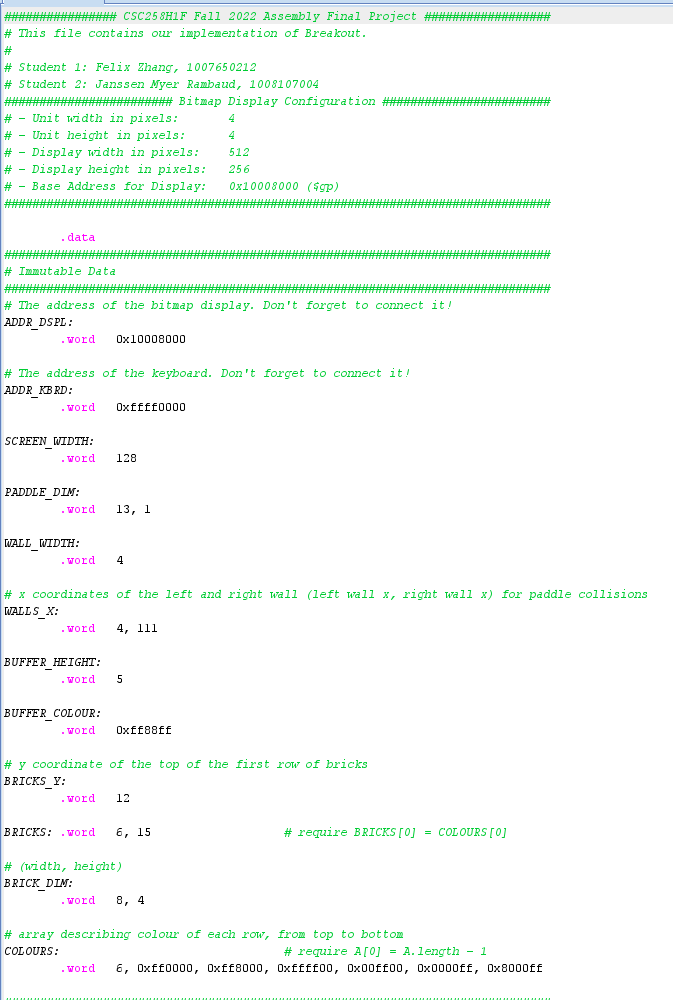
\includegraphics[width=0.5\textwidth]{memory2.png}
    \caption{Screenshot of .data code section (1).}
    \label{f:part1_memory1}
\end{figure}

\begin{figure}[ht!]
    \centering
    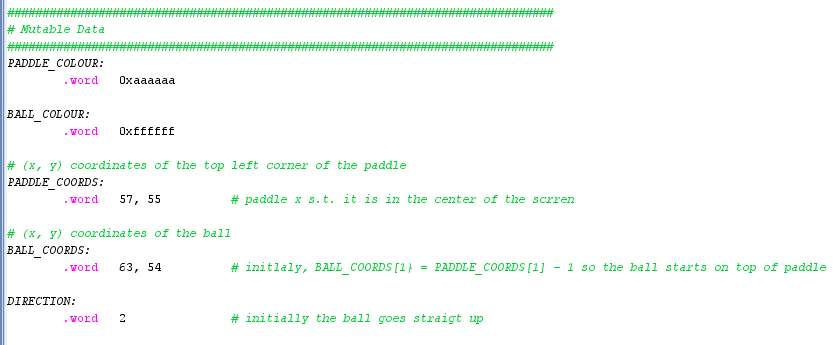
\includegraphics[width=0.5\textwidth]{memory3.png}
    \caption{Screenshot of .data code section (2).}
    \label{f:part1_memory2}
\end{figure}

\begin{figure}[ht!]
    \centering
    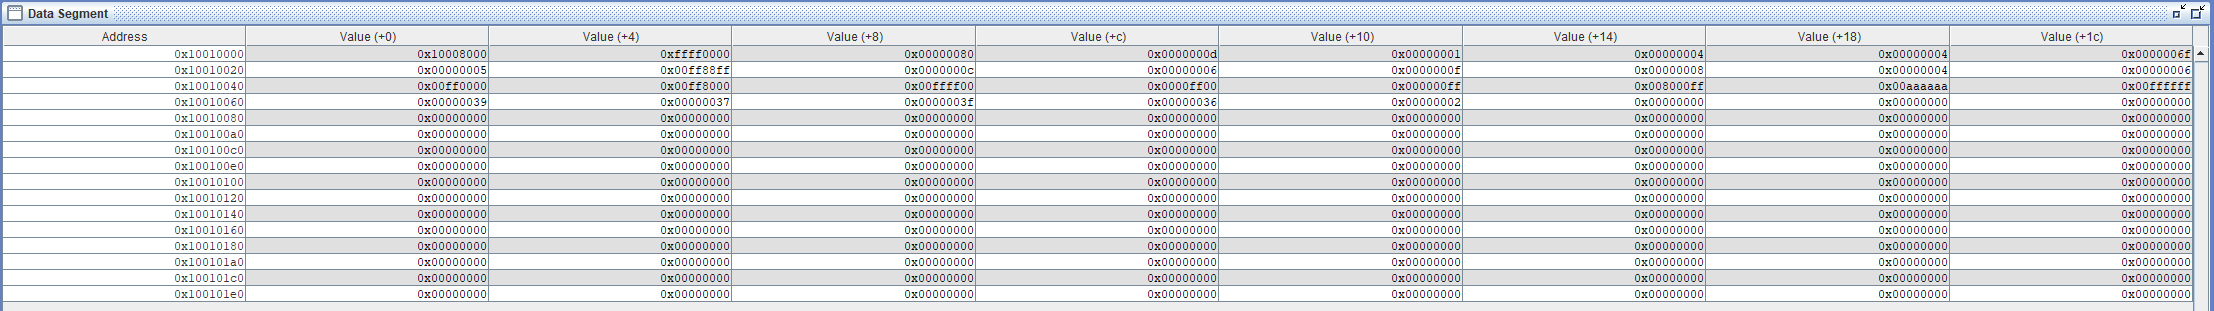
\includegraphics[width=1.2\textwidth]{memory1.png}
    \caption{Screenshot of .data memory.}
    \label{f:part1_memory3}
\end{figure}

\newpage

\section{Part II: Milestone 1}

\item Draw the scene (Milestone 1)

\begin{figure}[ht!]
    \centering
    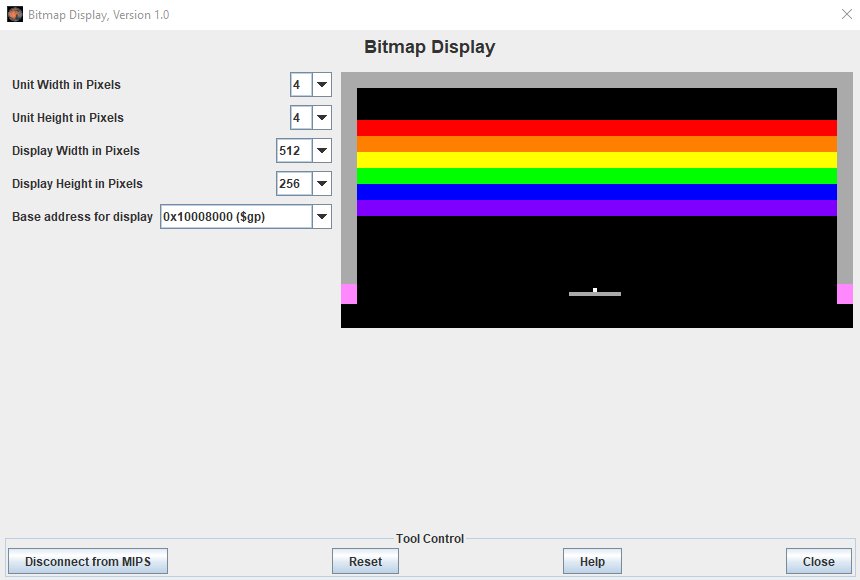
\includegraphics[width=0.8\textwidth]{milestone1_drawing.png}
    \caption{The static scene of Milestone 1 Drawing.}
    \label{f:milestone1_drawing}
\end{figure}

\end{enumerate}


\newpage

\section{Part III: Milestone 2}

\item \textbf{QUESTION: } How will the ball change directions when it collides? \\[0.4em]
The rules governing how the ball changes directions when it collides are as follows. \\[0.4em]
If it collided with the paddle, then the resulting direction depends on which section of the paddle it hit.
Hitting the leftmost third results it travelling north-east (at a $45^\circ$ angle), the middle third results it travelling north, and the rightmost third results in it travelling north-west (at a $45^\circ$ angle). \\[0.4em]
Otherwise, if it collided with a non-paddle object then the resulting direction depends on the original direction.
If the original direction of ball forms the angle $\theta$ with the surface it collided with, 
then the resulting direction is the reflection of the original direction across the line perpendicular to the collision surface away from the collision point.
For example, if the ball is travelling north-west (at a $45^\circ$ angle) and collides with the left wall, then it begins travelling in the north-east direction (at a $45^\circ$ angle).
Note this also means if the ball was travelling perpendicular to surface with which it collided, then after the collision, it is moving in the reverse direction.
So, if the ball was travelling north before colliding with the bottom of a brick, then it is travelling south after the collision.
\item Upload breakout.asm to MarkUs so that you have a snapshot of your progress so far.

\section{Part IV: Milestone 3}
\item Upload breakout.asm to MarkUs so that you have a snapshot of your progress so far.
\end{document}